\subsection{Audiowiedergabe durch PWM}\label{sec:audioPWM}
Nachdem der Zugriff und die Kommunikation mit der SD-Karte erklärt wurde, kann an dieser Stelle nun die Audiowiedergabe beschrieben werden. Damit ein Audiosignal abgespielt werden kann, sind zwei PWM-Signale Voraussetzung. Dabei ist das erste Signal das invertierte Signal des zweiten und umgekehrt. Abbildung \ref{fig:pwm_ausgang} zeigt das Prinzip.

\begin{figure}[H]
	\begin{center}
		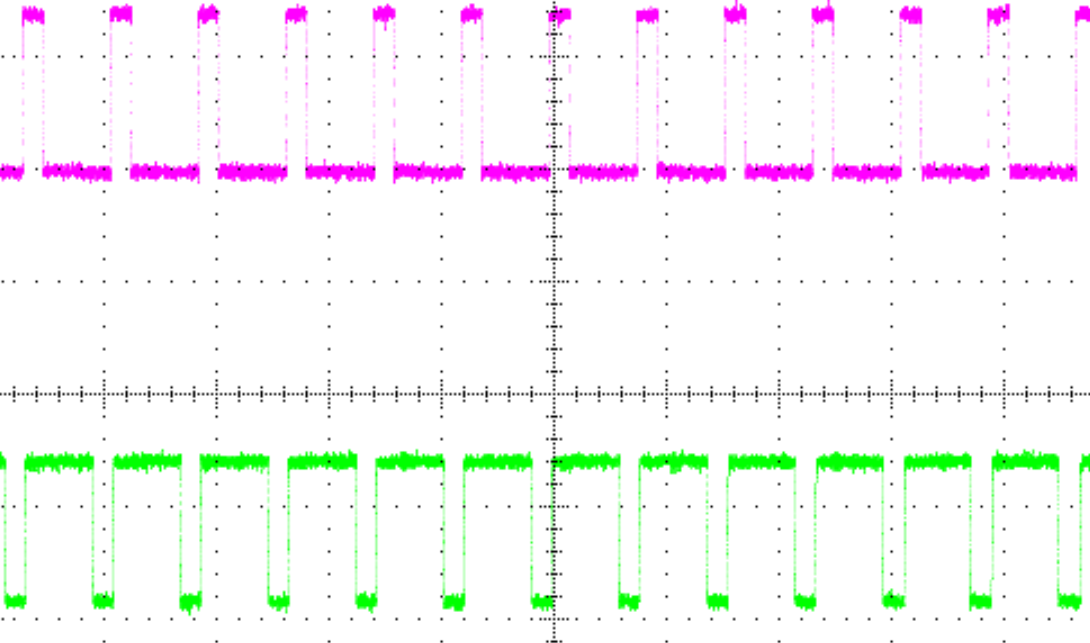
\includegraphics[width=0.7\textwidth]{data/PWM_Signal_500Hz_Mono}
		\caption[PWM-Ausgang des NRF52]{PWM-Ausgang des NRF52: Das violette Signal entspricht dem invertierten grünen Signal} %picture caption
		\label{fig:pwm_ausgang}
	\end{center}
\end{figure}

Das PWM-Signal wird mit dem NRF52-Controller generiert. NORDIC SEMICONDUCTOR stellt dafür die PWM HAL and driver Bibliothek zur Verfügung. Die genutzten Funktionen sind in der Tabelle \ref{table:bibliothek} aufgelistet. Der Controller bietet vier PWM-Instanzen mit je vier Kanälen. Für die Audioausgabe wurden zwei PWM-Instanzen mit je einem Kanal genutzt.

\begin{table}[H]
	\begin{center}
	\begin{tabular}{|l|l|l|}
		\hline
		%\rowcolor[HTML]{C0C0C0} 
		\textbf{Beschreibung} & \textbf{Funktion}                & \textbf{Argumente}                                                                                                                                                                                                            \\ \hline
		PWM initialisiern     & nrf\_drv\_pwm\_init              & \begin{tabular}[c]{@{}l@{}}nrf\_drv\_pwm\_t const *const p\_instance\\ nrf\_drv\_pwm\_config\_tconst *p\_config\\ nrf\_drv\_pwm\_handler\_thandler\end{tabular}                                                               \\ \hline
		Audio abspielen         & nrf\_drv\_pwm\_complex\_playback & \begin{tabular}[c]{@{}l@{}}nrf\_drv\_pwm\_t const *const p\_instance\\ nrf\_pwm\_sequence\_t const *p\_sequence\_0\\ nrf\_pwm\_sequence\_tconst *p\_sequence\_1\\ uint16\_t  playback\_count \\ uint32\_t  flags\end{tabular} \\ \hline
	\end{tabular}
	\caption[Funktionen der PWM HAL and driver Bibliothek]{Funktionen der PWM HAL and driver Bibliothek}
	\label{table:bibliothek}
\end{center}
\end{table}

Abbildung \ref{fig:pwm_ablauf} zeigt den Ablauf des PWM-Unterprogramms. Zuerst findet die Initialisierung statt. Anschliessend können die beiden Sequenzen 0 und 1 generiert werden, in welchen die Daten des Audio-Files abgelegt werden. Die Funktion complex\_playback generiert dann aufgrund der Sequenzen das entsprechende PWM-Signal am Ausgang. Nachfolgend werden die einzelnen Schritte noch detaillierter beschrieben.

\begin{figure}[H]
	\begin{center}
		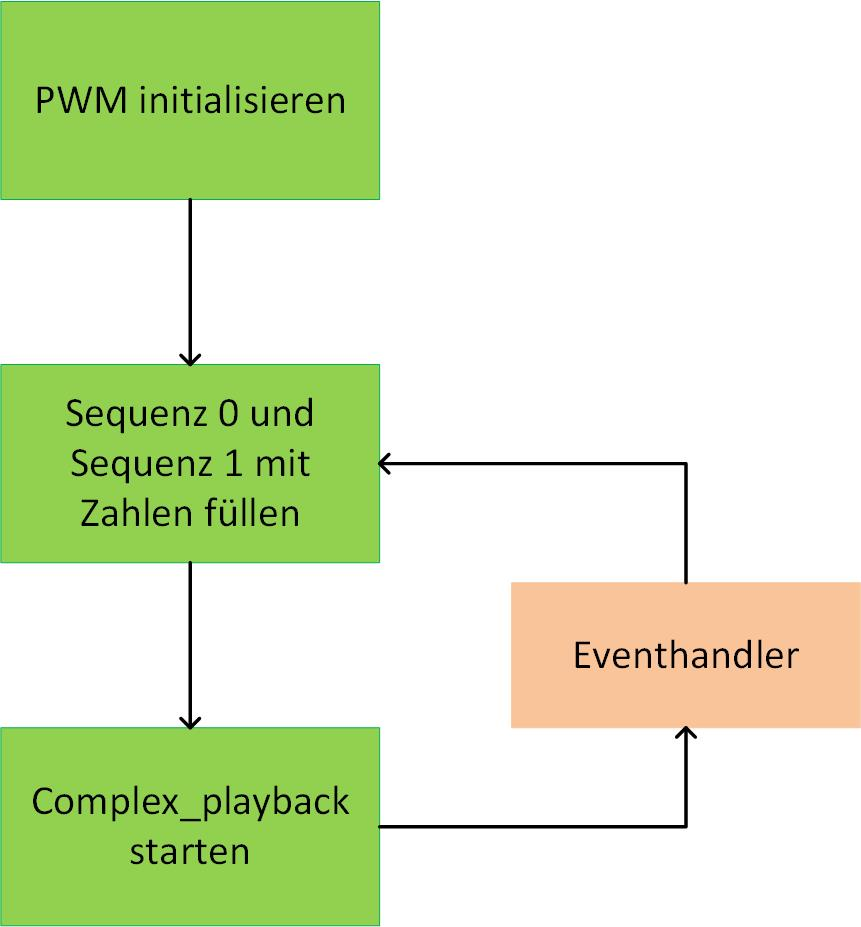
\includegraphics[width=0.5\textwidth]{data/pwm_ablauf}
		\caption[Ablauf PWM-Ausgabe]{Ablauf PWM-Ausgabe} %picture caption
		\label{fig:pwm_ablauf}
	\end{center}
\end{figure}

\subsubsection*{PWM Initialisieren}\label{sec:PWM initialisieren}
Bei der PWM-Initialisierung wurde die PWM-Instanz, die Config und der Eventhandler mitgegeben. Die Config des PWM musste anhand der Angaben des Wavefiles generiert werden. Die Werte wurden gemäss Tabelle \ref{table:config} gewählt.

\begin{table}[H]
	\centering
	\begin{tabular}{|l|l|l|}
	\hline
	\textbf{Parameter}  & \textbf{Gewählter Wert}    & \textbf{Bemerkung}                                                           \\ \hline
	output\_pins  & Pin 17                        & \begin{tabular}[c]{@{}l@{}} Pin 17 für PWM Modul 1                                                        \\ Pin 27 für PWM Modul 2 \end{tabular} 
	 \\ \hline
	irq\_priority & APP\_IRQ\_PRIORITY\_LOWEST & \begin{tabular}[c]{@{}l@{}} Wurde so gewählt, da keine \\ 	 anderen Interruptroutinen vorhanden \end{tabular} 
	 \\ \hline
	base\_clock   & NRF\_PWM\_CLK\_16MHz       & Es wurde die maximale clock Frequenz gewählt                                  \\ \hline
	count\_mode   & NRF\_PWM\_MODE\_UP         & PWM zählt bis zu top\_value
	 \\ \hline
	top\_value    & 500                        & Siehe Berechnung top\_value                                                            \\ \hline
	load\_mode    & NRF\_PWM\_LOAD\_COMMON     & \begin{tabular}[c]{@{}l@{}}Wurde gewählt, da alle PWM Kanäle \\ den selben Wert ausgeben\end{tabular} \\ \hline
	stepp\_mode   & NRF\_PWM\_STEP\_AUTO       &\begin{tabular}[c]{@{}l@{}} Jedes Sample wird gemäss der Anzahl \\ 	 definierter Wiederholungen abgespielt \end{tabular} 
	 \\ \hline
	\end{tabular}
	\caption{Gewählte Config Werte}
	\label{table:config}
\end{table}

\textbf{Berechnung top\_value}\\
Da die clock Frequenz (in Tabelle \ref{table:config}  base\_clock) des PWM Moduls auf $16MHz$ gesetzt wurde, beträgt der top\_value für eine Audiodatei mit Abtastfrequenz von $32kHz \;  500$. Dies berechnet sich wie folgt:
\begin{equation}
32kHz = \frac{16MHz}{top\_value}
 \Rightarrow \; top\_value = \frac{16MHz}{32kHz} = 500
\end{equation}

\subsubsection*{Sequenzen laden}\label{sec:Sequenzen befüllen}
Jetzt können die Sequenzen geladen werden. Mit der Funktion next\_Value werden neue Werte in die entsprechenden Sequenzen geladen. Diese Funktion ist im Kapitel \ref{sec:sdKarte} genauer beschrieben.

\subsubsection*{Complex playback}\label{sec:Complex playback}
Die Funktion generiert anhand der Sequenz ein entsprechendes PWM-Signal. Der
Vorteil zu simple playback ist, dass zwei Sequenzen mitgegeben werden können. Wenn die Sequenz 0 fertig abgespielt wurde, startet automatisch die zweite Sequenz und der Eventhandler wird ausgelöst. In dieser Zeit kann die erste Sequenz wieder neu beladen werden. Die Beladung der Sequenzen wird mit dem Eventhandler dieser Funktion gesteuert. 
